\lab{HIV Treatment Using Optimal Control}{HIV Treatment Using Optimal Control}
\label{lab:hiv}
\labdependencies{NumericalIVP}

\section*{Introduction}
Viruses cause many common illnesses in society today, including influenza, the common cold, and COVID-19. Viruses are obligate parasites, meaning that they must infect a host in order to replicate. After entering a host cell, viruses hijack host machinery to replicate their genome and translate their proteins. After this process, the new virus particles are assembled and lyse (break apart) the host cell to find a new host.

Mammalian immune systems are composed of two interconnected systems: the innate immune system and the adaptive immune system. While both branches of the immune system can combat viruses, the adaptive immune system is especially suited to recognize and neutralize viral infections. A major part of the adaptive immune response is helper T cells, as these cells moderate and regulate all other facets of the immune response. Helper T cells are most characterized by the presence of a receptor called CD4, which helps the cell recognize infections.  

One of the most devastating viral illnesses today is acquired immunodeficiency syndrome (AIDS), caused by the human immunodeficiency virus (HIV). HIV specifically targets and replicates in helper T cells, rendering them nonfunctional and killing them. By taking out the most important regulator of the immune system, HIV makes it difficult for the body to fight infection, so sicknesses that would normally be trivial for the body to manage, such as the common cold, yeast infections, and pneumonia, become deadly.

Currently, there is no cure for HIV, and vaccines are difficult to develop. Treatments that curb the replication of HIV and help maintain healthy helper T cell population levels are available, but they are expensive and must be taken for the rest of a patient’s life. Optimizing the dosage is essential to maximize the drug’s effect while minimizing the cost and negative side-effects of long-term usage. In this lab, we will use optimal control to find the optimum dosage of a two-drug combination to fight HIV.
In this lab we will use optimal control to find the optimal dosage of a two-drug combination\footnote{\textit{SHORT COURSES ON THE MATHEMATICS OF BIOLOGICAL COMPLEXITY}, Web. 15 Apr. 2015 http://www.math.utk.edu/~lenhart/smb2003.v2.html.}.
   
%\begin{problem}
%Explain what makes HIV unique. What are the consequences of this? What is AIDS?
%\label{problem:hiv:virusunderstanding}
%\end{problem}
%
%\begin{problem}
%How is AIDS treated and what are the considerations for treatment?
%\label{problem:hiv:treatment}
%\end{problem}

\section*{Derivation of Control}
We begin by defining some variables.
Let $T$ represents the concentration of $CD4^+T$ cells and $V$ the concentration of HIV particles.
$s_1$ and $s_2$ represent the production of T cells by various processes.
$B_1$ and $B_2$ are half saturation constants (sort of like crowd control in the blood stream and plasma).
Let $\mu$ be the death rate of uninfected T cells, k the rate of infection of T cells, and c the death rate of the virus.
Let g be the input rate of some external viral source.
The control variables $u_1$ and $u_2$ represent the amount of drugs that introduce new T cells or kill the virus, respectively.
\footnote{`Immunotherapy of HIV-1 Infection', Kirschner, D. and Webb, G. F., Journal of Biological Systems, 6(1), 71-83 (1998)}

Next we write the state system, the equations that describe the changes in T cells and viruses:
\begin{align}
	\begin{split}
		\frac{\it{d}T(t)}{\it{dt}} &= s_1 - \frac{s_2V(t)}{B_1+V(t)} - \mu T(t)-kV(t)T(t)+u_1(t)T(t), \\
		\frac{\it{d}V(t)}{\it{dt}} &= \frac{gV(t)}{B_2+V(t)}(1-u_2(t)) - cV(t)T(t).
	\end{split} \label{original_state:HIV}
\end{align}
The term $s_1-\frac{s_2V(t)}{B_1+V(t)}$ is the source/proliferation of unaffected T cells,
$\mu T(t)$ the natural loss of T cells, $kV(t)T(t)$ the loss of T cells by infection. 
$\frac{gV(t)}{B_2+V(t)}$ represents the viral contribution to plasma, and $cV(t)T(t)$ the viral loss.
To these equations we add initial conditions $T(0)=T_0$ and $V(0)=V_0$.
\footnote{`Optimal Control of an HIV Immunology Model', H.R Joshi}

We now seek to maximize the functional 
\[
J(u_1,u_2) = \int_0^{t_f}[T-(A_1u_1^2+A_2u_2^2)]\it{dt}.
\]
This functional considers i) the benefit of T cells, and ii) the systematic costs of drug treatments.
The constants $A_1$ and $A_2$ represent scalars to adjust the size of terms coming from $u_1^2$ and $u_2^2$ respectively. 
We seek an optimal control $u_1^*,u_2^*$ satisfying
\[
J(u_1^*,u_2^*)=\max_{(u_1,u_2)\in U}J(u_1,u_2) =\min_{(u_1,u_2)\in U}-J(u_1,u_2),
\]
where $U=\{(u_1,u_2):\,a_i\le u_i(t) \le b_i\text{ for }t\in[0,t_f], i=1,2\}$.
 
\section*{Optimality System}
The Hamiltonian is defined as:
\begin{align*}
	H = \vec{\lambda} \cdot \vec{f} - L\\
	H =\lambda_1\Big[ s_1 - \frac{s_2V}{B_1+V}-\mu T-kVT+u_1T \Big] &+ \lambda_2 \Big[\frac{g(1-u_2)V}{B_2+V}-cVT\Big]\\
	 &+  [T-(A_1u_1^2+A_2u_2^2)].
\end{align*}
Note that the costate is represented with $\lambda$ instead of $p$.
The costate evolution equations are:
\begin{align*}
	\lambda_1^{'} &=-\frac{\partial H}{\partial T} =  -1+\lambda_1[\mu+kV^*-u_1^*]+\lambda_2cV^*,\\
	\lambda_2^{'} &= -\frac{\partial H}{\partial V} = \lambda_1\Big[\frac{B_1s_2}{(B_1+V^*)^2}+kT^*\Big] -\lambda_2\Big[\frac{B_2g(1-u_2^*)}				{(B_2+V^*)^2}-cT^*\Big]
\end{align*}
where \(T^*, V^*\) denote the optimal \(T,V\).
The endpoint conditions are $\lambda_1(t_f)=\lambda_2(t_f)=0$, with $T(0)=T_0$ and $V(0)=V_0$. 
Using Pontryagin's maximum principle to find the control, we have
\begin{align*}
\frac{\partial H}{\partial u_1} &= -2A_1u_1^*(t)+\lambda_1T^*(t)=0
\frac{\partial H}{\partial u_2} &= -2A_2u_2^*(t)+\lambda_2\big[\frac{-gV^*(t)}{B_2+V^*(t)}\big]=0
\end{align*}
which gives (provided these are within the bounds of the controls)
\begin{align*}
	u_1^*(t) &= \frac{1}{2A_1}\left[\lambda_1T^*(t)\right],\\
	u_2^*(t) &= \frac{-1}{2A_2}\left[\lambda_2\frac{gV^*(t)}{B_2+V^*(t)}\right].
\end{align*}
Taking into account the bounds on the controls, we have
\begin{align*}
	\begin{split}
		u_1^*(t)&=\min\left\{\max\{a_1,\frac{1}{2A_1}(\lambda_1T^*(t))\},b_1\right\},\\
		u_2^*(t)&=\min\left\{\max\{a_2,\frac{-\lambda_2}{2A_2}\frac{gV^*(t)}{B_2+V^*(t)}\},b_2\right\}.
	\end{split}
\end{align*}
This gives us the optimal system
\begin{align}
	\begin{split}
		T'&=s_1-\frac{s_2V}{B_1+V}-\mu T-kVT+\min\{\max\{a_1,\frac{1}{2A_1}(\lambda_1T)\},b_1\}T,\\
		V'&=\frac{g(1-\min\{\max\{a_2,\frac{-\lambda_2}{2A_2}\frac{gV}{B_2+V}\},b_2\})V}{B_2+V}-cVT
	\end{split} \label{modified_state:HIV}\\
	\begin{split}
		\lambda_1'&=-1+\lambda_1\left[\mu+kV-\min\{\max\{a_1,\frac{1}{2A_1}(\lambda_1T)\},b_1\}\right]+\lambda_2cV,\\
		\lambda_2'&=\lambda_1\left[\frac{B_1s_2}{(B_1+V)^2}+kT\right]-\lambda_2\left[\frac{B_2g(1-\min\{\max\{a_2,\frac{-\lambda_2}{2A_2}\frac{V}			{B_2+V}\},b_2\})}{(B_2+V)^2}-cT\right],
	\end{split}
\end{align}
with end conditions $\lambda_1(t_f)=\lambda_2(t_f)=0$, and $T(0)=T_0,V(0)=V_0$.

\section*{Creating a Numerical Solver}

We iteratively solve for our control $u$.
In each iteration we solve our state equations and our costate equations numerically, then use those to find our new control.
Lastly, we check to see if our control has converged.
To solve each set of differential equations, we will use the RK4 solver from a previous lab with one minor adjustment.
Our state equations depend on $u$, and our costate equations depend on our state equations.
Therefore, we will pass another parameter into the function that RK4 takes in that will index the arrays our equations depend on.

\begin{lstlisting}
# Dependencies for this lab's code:
import numpy as np
from matplotlib import pyplot as plt

#Code from RK4 Lab with minor edits				
def initialize_all(y0, t0, tf, n):
    """ An initialization routine for the different ODE solving
    methods in the lab. This initializes Y, T, and h. """
    if isinstance(y0, np.ndarray):
        Y = np.empty((n, y0.size)).squeeze()
    else:
        Y = np.empty(n)
    Y[0] = y0
    T = np.linspace(t0, tf, n)
    h = float(tf - t0) / (n - 1)
    return Y, T, h

def RK4(f, y0, t0, tf, n):
    """ Use the RK4 method to compute an approximate solution
    to the ODE y' = f(t, y) at n equispaced parameter values from t0 to t
    with initial conditions y(t0) = y0.
    
    y0 is assumed to be either a constant or a one-dimensional numpy array.
    tf and t0 are assumed to be constants.
    f is assumed to accept three arguments.
    The first is a constant giving the value of t.
    The second is a one-dimensional numpy array of the same size as y.
    The third is an index to the other arrays.
    
    This function returns an array Y of shape (n,) if
    y is a constant or an array of size 1.
    It returns an array of shape (n, y.size) otherwise.
    In either case, Y[i] is the approximate value of y at
    the i'th value of np.linspace(t0, tf, n).
    """
    Y,T,h = initialize_all(y0,t0,tf,n)
    for i in range(n-1):
        K1 = f(T[i],Y[i],i)
        K2 = f(T[i]+h/2.,Y[i]+h/2.*K1,i)
        K3 = f(T[i]+h/2.,Y[i]+h/2.*K2,i)
        K4 = f(T[i+1],Y[i]+h*K3,i)
        Y[i+1] = Y[i] + h/6.*(K1+2*K2 +2*K3+K4)
    return Y
\end{lstlisting}

\begin{problem}
Create a function that defines the state equations and returns both equations in a single array. The function should be able to be passed into the RK4 solver. This function can depend on the global variables defined below.

\begin{warn}
When solving the state equations, because of the nature of $T^\prime$ and $V^\prime$, solve the original equations \eqref{original_state:HIV} from the beginning of the lab and not the equations \eqref{modified_state:HIV} with $u_i^*(t)$ replaced by the minmax function.
\end{warn}

\begin{lstlisting}
a_1, a_2 = 0, 0
b_1, b_2 = 0.02, 0.9
s_1, s_2 = 2., 1.5
mu = 0.002
k = 0.000025
g = 30.
c = 0.007
B_1, B_2 = 14, 1
A_1, A_2 = 250000, 75
T0, V0 = 400, 3
t_f = 50
n = 2000
\end{lstlisting}
These constants come from both references cited at the end of this lab. 

\begin{lstlisting}
# initialize global variables, state, costate, and u.
state = np.zeros((n,2))
state0 = np.array([T0, V0])
	
costate = np.zeros((n,2))
costate0 = np.zeros(2)

u=np.zeros((n,2))
u[:,0] = .02
u[:,1] = .9

# define state equations
def state_equations(t,y,i):
	'''
	Parameters
	---------------
	t : float
		the time
	y : ndarray (2,)
		the T cell concentration and the Virus concentration at time t
	i : int
		index for the global variable u.
	Returns
	--------------
	y_dot : ndarray (2,)
		the derivative of the T cell concentration and the virus concentration at time t
	'''
	pass
\end{lstlisting}
\label{problem:hiv:state}
\end{problem}


The state equations work great in the RK4 solver; however, the costate equations have end conditions rather than initial conditions. Thus we want our RK4 solver to iterate backwards from the end to the beginning. An easy way to accomplish this is to define a function $ \hat{\lambda}_i(t)=\lambda_i(t_f - t).$ Then $\hat{\lambda}_i$ has the initial conditions $\hat{\lambda}_i(0) = \lambda_i(t_f)$. We get the new equations

\begin{align*}
\hat{\lambda}_1'(t) &=\lambda_1(t_f-t)\left(-\mu - kV(t_f-t) + u_{1}(t_f-t)\right) - c\lambda_2(t_f-t)V(t_f-t) + 1, \\
\hat{\lambda}_2'(t) &= -\lambda_1(t_f-t)\left(\frac{s_2B_1}{(B_1+V(t_f-t))^2}+kT(t_f-t)\right) \\
&\quad+ \lambda_2(t_f-t)\left(\frac{gB_2(1-u_2(t_f-t))}{(B_2 + V(t_f-t))^2} - cT(t_f-t)\right).
\end{align*}

These we can solve with our RK4 solver and recover the original costate equations by simply indexing the array backwards.

\begin{problem}
Create a function that defines the costate equations and returns both equations in a single array. The function should be able to be passed into the RK4 solver. Use the global variables as defined in Problem \ref{problem:hiv:state}.

\begin{lstlisting}
def lambda_hat(t,y,i):
	'''
	Parameters
	---------------
	t : float
		the time
	y : ndarray (2,)
		the lambda_hat values at time t
	i : int
		index for global variables, u and state.
	Returns
	--------------
	y_dot : ndarray (2,)
		the derivative of the lambda_hats at time t.
	'''
	pass
\end{lstlisting}

\label{problem:hiv:costateequations}
\end{problem}


\begin{figure}
\centering
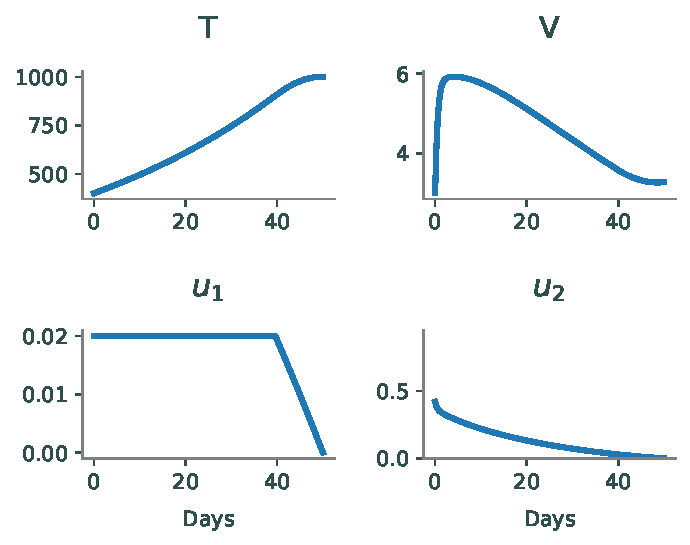
\includegraphics[width=5in]{figures/hiv_solution.pdf}
\caption{The solution to Problem \ref{problem:hiv:numericalsolver}.}
\label{fig:hiv:solutions}
\end{figure}



Finally, we can put these together to create our solver.
\begin{problem}
Create and run a numerical solver for the HIV two drug model using the code below.

\begin{lstlisting}
epsilon = 0.001
test = epsilon + 1

while(test > epsilon):
	oldu = u.copy();
    
	#solve the state equations with forward iteration
	#state = RK4(...)
    
	#solve the costate equations with backwards iteration
	#costate = RK4(...)[::-1]
	
	#solve for u1 and u2
    
	#update control
	u[:,0] = 0.5*(u1 + oldu[:,0])
	u[:,1] = 0.5*(u2 + oldu[:,1])

	#test for convergence
	test = abs(oldu - u).sum()
\end{lstlisting}

Your solutions should match Figure \ref{fig:hiv:solutions}.
\label{problem:hiv:solver}

\label{problem:hiv:numericalsolver}
\end{problem}

Patients usually take several different classes of drugs at a time to prevent HIV from replicating and progressing into AIDS. Reverse transcriptase inhibitors prevent the HIV genome from inserting itself into the host genome. These prevent helper T cell death by lowering the number of HIV particles in the body. Protease inhibitors prevent the activation of HIV proteins that are needed for replication. Fusion inhibitors can be taken early in the course of HIV infection and prevent the entry of HIV into helper T cells. 
There are many unique drugs in each class, all with known and unknown interactions and side effects. Physicians rotate through drugs to help their patients have a positive outcome and to prevent the virus from becoming resistant to any one drug.

% \begin{thebibliography}{9}
%
% \bibitem{paper}
% "SHORT COURSES ON THE MATHEMATICS OF BIOLOGICAL COMPLEXITY." \textit{SHORT COURSES ON THE MATHEMATICS OF BIOLOGICAL COMPLEXITY}. Web. 15 Apr. 2015. http://www.math.utk.edu/~lenhart/smb2003.v2.html.
%
% \bibitem{constants}
% Kirschner, D. and Webb, G. F., `Immunotherapy of HIV-1 Infection', Journal of Biological Systems, 6(1), 71-83 (1998).
% \end{thebibliography}